%%%%%%%%%%%%%%%%%%%%%%% file template.tex %%%%%%%%%%%%%%%%%%%%%%%%%
%
% This is a general template file for the LaTeX package SVJour3
% for Springer journals.          Springer Heidelberg 2010/09/16
%
% Copy it to a new file with a new name and use it as the basis
% for your article. Delete % signs as needed.
%
% This template includes a few options for different layouts and
% content for various journals. Please consult a previous issue of
% your journal as needed.
%
%%%%%%%%%%%%%%%%%%%%%%%%%%%%%%%%%%%%%%%%%%%%%%%%%%%%%%%%%%%%%%%%%%%
%
% First comes an example EPS file -- just ignore it and
% proceed on the \documentclass line
% your LaTeX will extract the file if required
\begin{filecontents*}{example.eps}
%!PS-Adobe-3.0 EPSF-3.0
%%BoundingBox: 19 19 221 221
%%CreationDate: Mon Sep 29 1997
%%Creator: programmed by hand (JK)
%%EndComments
gsave
newpath
  20 20 moveto
  20 220 lineto
  220 220 lineto
  220 20 lineto
closepath
2 setlinewidth
gsave
  .4 setgray fill
grestore
stroke
grestore
\end{filecontents*}
%
\RequirePackage{fix-cm}
%
\documentclass{svjour3}                     % onecolumn (standard format)
%\documentclass[smallcondensed]{svjour3}     % onecolumn (ditto)
%\documentclass[smallextended]{svjour3}       % onecolumn (second format)
%\documentclass[twocolumn]{svjour3}          % twocolumn
%
\smartqed  % flush right qed marks, e.g. at end of proof
%
\usepackage{mhsetup}
\usepackage{amsmath}
\usepackage{mathtools}
\usepackage{natbib}
\usepackage{graphicx}
\usepackage{float}
\usepackage{qtree}
\usepackage[utf8]{inputenc}
\usepackage{gb4e}
\usepackage[T1]{fontenc}
\usepackage{ tipa }
\bibpunct{(}{)}{,}{a}{}{,}
\newcommand{\noteme}[1]{\noindent \textbf{[[JCW:  #1 ]]}}
\renewcommand{\theequation}{\Alph{equation}}

% Insert the name of "your journal" with
\journalname{Journal of }

\begin{document}

\title{Three Ways Allophonic Rules Emerge
\thanks{people}}
%\subtitle{Do you have a subtitle?\\ If so, write it here}

%\titlerunning{Short form of title}        % if too long for running head

\author{Betsy Sneller and Joel C. Wallenberg and ?}

%\authorrunning{Short form of author list} % if too long for running head

\institute{Joel C. Wallenberg \at
              Newcastle University \\
              Tel.: +44-(0)191-222-7366\\
              \email{joel.wallenberg@ncl.ac.uk}
}

\date{Received: date / Accepted: date}
% The correct dates will be entered by the editor


\maketitle

\begin{abstract}
stuff
\keywords{phonology \and language change \and allophony \and sociolinguistics}
% \PACS{PACS code1 \and PACS code2 \and more}
% \subclass{MSC code1 \and MSC code2 \and more}
\end{abstract}

\section{Introduction}
\label{intro}

We are now reaching the point in the fields of language change, sociolinguistics, and language acquisition where we can go well beyond Neogrammarian descriptions of sound change, and even beyond the influential work by Kiparsky \noteme{get refs}, to ask nuanced questions about how phonological systems emerge. This is to say that we can now treat the ``actuation problem'' as more than just a problem \citep{wlh1968}: it is a research program, with hypotheses posed at a high level of detail.

Our hypothesis is that there are three distinct possible diachronic paths to allophony, all of which may be currently attested:
\begin{enumerate}
    \item The traditionally assumed scenario, recently elaborated by Burmudez-Otero \noteme{get refs}: a low-level phonetic, articulatory, or acoustic/perceptual effect created by a phonotactic context becomes strong enough to be phonologized, reanalyzed at some point by learners as an allophonic rule. 
    \item Speakers spontaneously create an allophone without any phonetic motivation: speakers split one phonological category into two through a pure reanalysis, creating an allophone with no initial phonetic difference from the other allophone. Subsequently, over generational time, the two purely phonological allophones diverge phonetically.
    \item A purely phonetic change begins, creating variation in phonetic space, and then different sections of this variation being to specialize for different phonological contexts over time. The phonological change occurs as a reanalysis of the ``old'' and ``new'' variants of a phonetic change in progress, after that change is well underway (for independent reasons).
\end{enumerate}
\noindent We present evidence below suggesting that all of these scenarios have occurred in the histories of languages, but we do not pretend that this article will settle the question definitively. Rather, we intend the present discussion as a challenge to the fields of historical phonology and sociolinguistics to either confirm or falsify these hypotheses, or to show that some of these scenarios can in fact be reduced to one of the others.

In the first section below, we present some evidence showing that contextual phonetic effects can be reanalyzed as phonological rules. (As there is already a large literature on this topic, we only select a few clear examples.) In section \ref{newzea}, we present new data from an ongoing sound change in New Zealand English illustrating that an allophonic split can occur in the middle of an originally unconditioned sound change in progress. Section \ref{philly} reviews and builds on a potentially revolutionary result from \citet{fruehwald2013}, showing that allophonic split can also occur in the absence of any phonetic contextual effects, as a ``pure'' reanalysis. Finally, section \ref{test} proposes some ways in which the field can test and attempt to falsify the hypotheses presented in this paper.

%1) A "traditional"ly recognized situation: which really seems to be the case for certain types of consonant allophony, like n -> velar / _ velar. This is the case where the allophones seem to match their environments phonotactically, and so it's likely that phonetic aspects of the context really created the allophones.

%2) The "Joe"-type change: speakers spontaneously reanalyze one phonological category as 2, creating an allophone with no initial phonetic difference. Then the two purely phonological allophones subsequently diverge phonetically, as in /ai/-raising in Philly (perhaps driven by the Principle of Contrast -- two phonological forms with the same phonetic target is unstable, so they specialize for different phonetic targets over time). Here the phonological change is prior to the phonetic one.

%3) The "Betsy"-type change: a phonetic change begins, creating variation in phonetic space, and then different sections of this variation being to specialize for different phonological contexts, starting a phonological change *after* the initial phonetic change has already begun.

\section{Life Cycle of Phonological Processes}
\label{trad}

%Cite Ricardo a lot, and Danielle



\section{}
\label{newzea}

\section{}
\label{philly}

We build on \citet{fruehwald2013} analysis of his important result by suggesting that the phonetic change which follows the phonological reanalysis can be explained by general principles of language acquisition.


\section{Invitation to Falsification}
\label{test}


\section{Conclusions}



Hi I'm betsy testing git




% For one-column wide figures use
%\begin{figure}
% Use the relevant command to insert your figure file.
% For example, with the graphicx package use
%  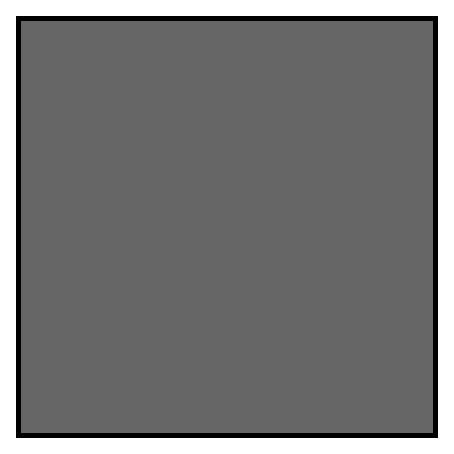
\includegraphics{example.eps}
% figure caption is below the figure
%\caption{Please write your figure caption here}
%\label{fig:1}       % Give a unique label
%\end{figure}
%
% For two-column wide figures use
%\begin{figure*}
% Use the relevant command to insert your figure file.
% For example, with the graphicx package use
%  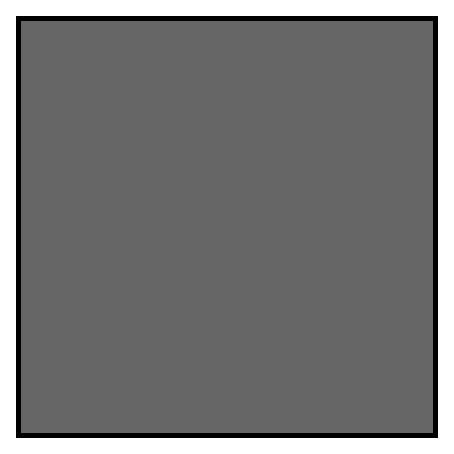
\includegraphics[width=0.75\textwidth]{example.eps}
% figure caption is below the figure
%\caption{Please write your figure caption here}
%\label{fig:2}       % Give a unique label
%\end{figure*}
%
% For tables use
%\begin{table}
% table caption is above the table
%\caption{Please write your table caption here}
%\label{tab:1}       % Give a unique label
% For LaTeX tables use
%\begin{tabular}{lll}
%\hline\noalign{\smallskip}
%first & second & third  \\
%\noalign{\smallskip}\hline\noalign{\smallskip}
%number & number & number \\
%number & number & number \\
%\noalign{\smallskip}\hline
%\end{tabular}
%\end{table}


%\begin{acknowledgements}

%\end{acknowledgements}

% BibTeX users please use one of
%\bibliographystyle{spbasic}      % basic style, author-year citations
%\bibliographystyle{spmpsci}      % mathematics and physical sciences
%\bibliographystyle{spphys}       % APS-like style for physics
\bibliographystyle{linquiry2} %use spbasic for journal of comparative gmc linguistics, etc.
\bibliography{../joelrefs}   % name your BibTeX data base

\end{document}
% end of file template.tex

 